\documentclass[doc]{apa6}

\usepackage{amssymb,amsmath}
\usepackage{ifxetex,ifluatex}
\usepackage{fixltx2e} % provides \textsubscript
\ifnum 0\ifxetex 1\fi\ifluatex 1\fi=0 % if pdftex
  \usepackage[T1]{fontenc}
  \usepackage[utf8]{inputenc}
\else % if luatex or xelatex
  \ifxetex
    \usepackage{mathspec}
    \usepackage{xltxtra,xunicode}
  \else
    \usepackage{fontspec}
  \fi
  \defaultfontfeatures{Mapping=tex-text,Scale=MatchLowercase}
  \newcommand{\euro}{€}
\fi
% use upquote if available, for straight quotes in verbatim environments
\IfFileExists{upquote.sty}{\usepackage{upquote}}{}
% use microtype if available
\IfFileExists{microtype.sty}{\usepackage{microtype}}{}

% Table formatting
\usepackage{longtable, booktabs}
\usepackage{lscape}
% \usepackage[counterclockwise]{rotating}   % Landscape page setup for large tables
\usepackage{multirow}		% Table styling
\usepackage{tabularx}		% Control Column width
\usepackage[flushleft]{threeparttable}	% Allows for three part tables with a specified notes section
\usepackage{threeparttablex}            % Lets threeparttable work with longtable

% Create new environments so endfloat can handle them
% \newenvironment{ltable}
%   {\begin{landscape}\begin{center}\begin{threeparttable}}
%   {\end{threeparttable}\end{center}\end{landscape}}

\newenvironment{lltable}
  {\begin{landscape}\begin{center}\begin{ThreePartTable}}
  {\end{ThreePartTable}\end{center}\end{landscape}}

  \usepackage{ifthen} % Only add declarations when endfloat package is loaded
  \ifthenelse{\equal{\string doc}{\string man}}{%
   \DeclareDelayedFloatFlavor{ThreePartTable}{table} % Make endfloat play with longtable
   % \DeclareDelayedFloatFlavor{ltable}{table} % Make endfloat play with lscape
   \DeclareDelayedFloatFlavor{lltable}{table} % Make endfloat play with lscape & longtable
  }{}%



% The following enables adjusting longtable caption width to table width
% Solution found at http://golatex.de/longtable-mit-caption-so-breit-wie-die-tabelle-t15767.html
\makeatletter
\newcommand\LastLTentrywidth{1em}
\newlength\longtablewidth
\setlength{\longtablewidth}{1in}
\newcommand\getlongtablewidth{%
 \begingroup
  \ifcsname LT@\roman{LT@tables}\endcsname
  \global\longtablewidth=0pt
  \renewcommand\LT@entry[2]{\global\advance\longtablewidth by ##2\relax\gdef\LastLTentrywidth{##2}}%
  \@nameuse{LT@\roman{LT@tables}}%
  \fi
\endgroup}


  \usepackage{graphicx}
  \makeatletter
  \def\maxwidth{\ifdim\Gin@nat@width>\linewidth\linewidth\else\Gin@nat@width\fi}
  \def\maxheight{\ifdim\Gin@nat@height>\textheight\textheight\else\Gin@nat@height\fi}
  \makeatother
  % Scale images if necessary, so that they will not overflow the page
  % margins by default, and it is still possible to overwrite the defaults
  % using explicit options in \includegraphics[width, height, ...]{}
  \setkeys{Gin}{width=\maxwidth,height=\maxheight,keepaspectratio}
\ifxetex
  \usepackage[setpagesize=false, % page size defined by xetex
              unicode=false, % unicode breaks when used with xetex
              xetex]{hyperref}
\else
  \usepackage[unicode=true]{hyperref}
\fi
\hypersetup{breaklinks=true,
            pdfauthor={},
            pdftitle={Evaluating Content-Related Validity Evidence Using Text Modeling},
            colorlinks=true,
            citecolor=blue,
            urlcolor=blue,
            linkcolor=black,
            pdfborder={0 0 0}}
\urlstyle{same}  % don't use monospace font for urls

\setlength{\parindent}{0pt}
%\setlength{\parskip}{0pt plus 0pt minus 0pt}

\setlength{\emergencystretch}{3em}  % prevent overfull lines


% Manuscript styling
\captionsetup{font=singlespacing,justification=justified}
\usepackage{csquotes}
\usepackage{upgreek}



\usepackage{tikz} % Variable definition to generate author note

% fix for \tightlist problem in pandoc 1.14
\providecommand{\tightlist}{%
  \setlength{\itemsep}{0pt}\setlength{\parskip}{0pt}}

% Essential manuscript parts
  \title{Evaluating Content-Related Validity Evidence Using Text Modeling}

  \shorttitle{Text Modeling Validity}


  \author{Daniel Anderson\textsuperscript{1}, Brock Rowley\textsuperscript{1}, \& Sondra Stegenga\textsuperscript{1}}

  % \def\affdep{{"", "", ""}}%
  % \def\affcity{{"", "", ""}}%

  \affiliation{
    \vspace{0.5cm}
          \textsuperscript{1} University of Oregon  }

  \authornote{
    Correspondence concerning this article should be addressed to Daniel
    Anderson, 5262 University of Oregon. E-mail:
    \href{mailto:daniela@uoregon.edu}{\nolinkurl{daniela@uoregon.edu}}
  }


  \abstract{Topic modeling is applied with science content standards to evaluate
semantic clustering. The probability that each item from a statewide
assessment belongs to each cluster/topic is then estimated as a source
of content-related validity evidence. We also show how visualizations
can map the content coverage of the test.}
  




\usepackage{amsthm}
\newtheorem{theorem}{Theorem}[section]
\newtheorem{lemma}{Lemma}[section]
\theoremstyle{definition}
\newtheorem{definition}{Definition}[section]
\newtheorem{corollary}{Corollary}[section]
\newtheorem{proposition}{Proposition}[section]
\theoremstyle{definition}
\newtheorem{example}{Example}[section]
\theoremstyle{definition}
\newtheorem{exercise}{Exercise}[section]
\theoremstyle{remark}
\newtheorem*{remark}{Remark}
\newtheorem*{solution}{Solution}
\begin{document}

\maketitle

\setcounter{secnumdepth}{0}



\hypertarget{conceptual-framework}{%
\subsection{Conceptual Framework}\label{conceptual-framework}}

Content-related validity evidence is a critical component of the
\enquote{overall evaluative judgment} (Messick, 1995, p. 741) of the
validity of test scores for a given use, and is one of the five major
sources of validity evidence outlined by the \emph{Standards for
Educational and Psychological Testing} (A. E. R. Association,
Association, Measurement in Education, \& others, 2014). Empirical
evaluations of of content validity evidence for high-stakes tests
generally come in the form of alignment studies, with panels of experts
judging the alignment match between the content represented within the
test items and the content represented in the corresponding standards
(Sireci, 2007; Webb, 1997). In this presentation, we explore the use of
text-mining procedures to evaluate the language used within the content
standards and the corresponding language used in the test items (i.e.,
the item stems and response options). We demonstrate that these
procedures can be successfully applied to not only identify
correspondence between items and standards, but also to evaluate the
content coverage and standards representation across the items.

\hypertarget{methods}{%
\subsection{Methods}\label{methods}}

Our particular application corresponds to evaluating the
content-validity evidence for the statewide alternate assessment based
on alternate achievement standards (AA-AAS) for student with the most
significant cognitive disabilities (United States Department of
Education, 2005) in one western state. We evaluate the concurrence
between the text in the Grade 8 \emph{Next Generation Science Standards}
(NGSS) and the text in the item stems and response options for the
corresponding statewide AA-AAS. As Ysseldyke and Olsen (1997) note,
\enquote{There is more variability in the skill levels and needs of this
1\% of the students than there is in the rest of the total student
population} (p.~16). Correspondingly, the development of items followed
a staged process, where content standards were first identified, and
then three versions of essentially the same item were developed to be
of, theoretically, \emph{low}, \emph{medium}, and \emph{high}
difficulty. In science, key vocabulary is a critical component of
demonstrating knowledge and all \emph{high} items were written to
include this vocabulary. However, this was not the case for the
\emph{low} or \emph{medium} items and we therefore presumed, a priori,
that the textual match of the \emph{high} items with the content
standards would be greater than the \emph{low} or \emph{medium} items.

In evaluating the concordance between the language used in the content
standards and the language used in the test items, our approach is to
use a text-based machine learning model, specifically topic modeling
\textbf{(CITE)}, to mine the standards and evaluate the topics
represented therein. Once this model is trained, we can estimate the
probability that each item is represented by each topic. In other words,
the model learns the patterns of words from the standards, and we can
then evaluate whether the words used in the items correspond to those
patterns.

Topic modeling is akin to exploratory factor analysis, where word
clusters (topics) are determined based on their semantic coherence
\textbf{(CITE)}. Post-hoc investigations of the topics then provide
substantive meaning. In our investigation, we expected seven topics to
emerge, which generally correspond to the sub-domains represented in the
Grade 8 NGSS standards.

Latent Dirichlet Allocation (LDA) was used\ldots{} \textbf{(CITE)}. We
removed stop words according to\ldots{} \textbf{(CITE)}.

Data were analyzed using using R (R Core Team, 2018) with the
\emph{textmodeling} package (Grün \& Hornik, 2011). All code used for
the analyses will be made publicly available.

\hypertarget{preliminary-results}{%
\subsection{Preliminary Results}\label{preliminary-results}}

\hypertarget{conclusions-and-implications}{%
\subsection{Conclusions and
Implications}\label{conclusions-and-implications}}

Overall, this paper will discuss a new and innovative proposed approach
to establishing validity through analyzing and categorizing text data
via modern data tools of R and RStudio text analysis and structural
topic modeling. It does not replace current methods for establishing
validity but demonstrates initial promise to add strength to the
development design. In a world of constantly evolving and growing data
and data sources it is imperative as educational researchers that we not
only begin to explore new methods that hold promise for increasing
efficiency and accuracy with data analysis but also ensure that methods
engage an element of translatability. By increasing the accuracy of
constructs and improved validity we provide the opportunity to increase
utility and translatability over a range of consumers in the educational
community. In addition, modern technology provides an array of methods
and open source resources and tools, such as R and RStudio, that not
only provide the ability to capture and categorize the data but also
visualize the findings. Again, this is an imperative piece in a world
that has seen vastly increased calls for the translation of data and
research to practice and practice to research.

\newpage

\hypertarget{references}{%
\section{References}\label{references}}

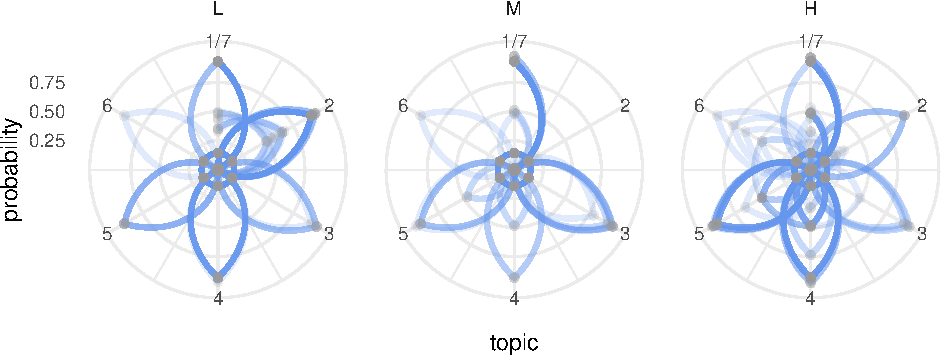
\includegraphics{ncme19_files/figure-latex/modeling-1.pdf}

\hypertarget{refs}{}
\leavevmode\hypertarget{ref-standards14}{}%
Association, A. E. R., Association, A. P., Measurement in Education, N.
C. on, \& others. (2014). AERA, apa, \& ncme. \emph{Standards for
Educational and Psychological Testing. Washington, DC: American
Educational Research Association}.

\leavevmode\hypertarget{ref-grun11}{}%
Grün, B., \& Hornik, K. (2011). topicmodels: An R package for fitting
topic models. \emph{Journal of Statistical Software}, \emph{40}(13),
1--30.
doi:\href{https://doi.org/10.18637/jss.v040.i13}{10.18637/jss.v040.i13}

\leavevmode\hypertarget{ref-messick95}{}%
Messick, S. (1995). Validity of psychological assessment: Validation of
inferences from persons' responses and performances as scientific
inquiry into score meaning. \emph{American Psychologist}, \emph{50}(9),
741.

\leavevmode\hypertarget{ref-r}{}%
R Core Team. (2018). \emph{R: A language and environment for statistical
computing}. Vienna, Austria: R Foundation for Statistical Computing.
Retrieved from \url{https://www.R-project.org/}

\leavevmode\hypertarget{ref-sireci07}{}%
Sireci, S. G. (2007). On validity theory and test validation.
\emph{Educational Researcher}, \emph{36}(8), 477--481.

\leavevmode\hypertarget{ref-usdoe05}{}%
United States Department of Education. (2005). \emph{Alternate
achievement standards for students with the most significant cognitive
disabilities: Non-regulatory guidance}. Retrieved from
\url{https://www2.ed.gov/policy/elsec/guid/altguidance.doc}

\leavevmode\hypertarget{ref-webb97}{}%
Webb, N. L. (1997). Criteria for alignment of expectations and
assessments in mathematics and science education. Research monograph no.
6.

\leavevmode\hypertarget{ref-ysseldyke97}{}%
Ysseldyke, J. E., \& Olsen, K. (1997). Putting alternate assessments
into practice: What to measure and possible sources of data (nceo
synthesis reports).






\end{document}
